% Options for packages loaded elsewhere
\PassOptionsToPackage{unicode}{hyperref}
\PassOptionsToPackage{hyphens}{url}
%
\documentclass[
]{article}
\author{}
\date{}

\usepackage{amsmath,amssymb}
\usepackage{lmodern}
\usepackage{iftex}
\ifPDFTeX
  \usepackage[T1]{fontenc}
  \usepackage[utf8]{inputenc}
  \usepackage{textcomp} % provide euro and other symbols
\else % if luatex or xetex
  \usepackage{unicode-math}
  \defaultfontfeatures{Scale=MatchLowercase}
  \defaultfontfeatures[\rmfamily]{Ligatures=TeX,Scale=1}
\fi
% Use upquote if available, for straight quotes in verbatim environments
\IfFileExists{upquote.sty}{\usepackage{upquote}}{}
\IfFileExists{microtype.sty}{% use microtype if available
  \usepackage[]{microtype}
  \UseMicrotypeSet[protrusion]{basicmath} % disable protrusion for tt fonts
}{}
\makeatletter
\@ifundefined{KOMAClassName}{% if non-KOMA class
  \IfFileExists{parskip.sty}{%
    \usepackage{parskip}
  }{% else
    \setlength{\parindent}{0pt}
    \setlength{\parskip}{6pt plus 2pt minus 1pt}}
}{% if KOMA class
  \KOMAoptions{parskip=half}}
\makeatother
\usepackage{xcolor}
\IfFileExists{xurl.sty}{\usepackage{xurl}}{} % add URL line breaks if available
\IfFileExists{bookmark.sty}{\usepackage{bookmark}}{\usepackage{hyperref}}
\hypersetup{
  hidelinks,
  pdfcreator={LaTeX via pandoc}}
\urlstyle{same} % disable monospaced font for URLs
\usepackage{longtable,booktabs,array}
\usepackage{calc} % for calculating minipage widths
% Correct order of tables after \paragraph or \subparagraph
\usepackage{etoolbox}
\makeatletter
\patchcmd\longtable{\par}{\if@noskipsec\mbox{}\fi\par}{}{}
\makeatother
% Allow footnotes in longtable head/foot
\IfFileExists{footnotehyper.sty}{\usepackage{footnotehyper}}{\usepackage{footnote}}
\makesavenoteenv{longtable}
\usepackage{graphicx}
\makeatletter
\def\maxwidth{\ifdim\Gin@nat@width>\linewidth\linewidth\else\Gin@nat@width\fi}
\def\maxheight{\ifdim\Gin@nat@height>\textheight\textheight\else\Gin@nat@height\fi}
\makeatother
% Scale images if necessary, so that they will not overflow the page
% margins by default, and it is still possible to overwrite the defaults
% using explicit options in \includegraphics[width, height, ...]{}
\setkeys{Gin}{width=\maxwidth,height=\maxheight,keepaspectratio}
% Set default figure placement to htbp
\makeatletter
\def\fps@figure{htbp}
\makeatother
\setlength{\emergencystretch}{3em} % prevent overfull lines
\providecommand{\tightlist}{%
  \setlength{\itemsep}{0pt}\setlength{\parskip}{0pt}}
\setcounter{secnumdepth}{-\maxdimen} % remove section numbering
\ifLuaTeX
  \usepackage{selnolig}  % disable illegal ligatures
\fi

\begin{document}

\hypertarget{ux57faux4e8eux51b3ux7b56ux7684ux9ed1ux76d2ux6587ux672cux5bf9ux6297ux6837ux672cux653bux51fbux65b9ux6848ux7814ux7a76ux4e0eux5b9eux73b0}{%
\section{\texorpdfstring{\textbf{基于决策的黑盒文本对抗样本攻击方案研究与实现}}{基于决策的黑盒文本对抗样本攻击方案研究与实现}}\label{ux57faux4e8eux51b3ux7b56ux7684ux9ed1ux76d2ux6587ux672cux5bf9ux6297ux6837ux672cux653bux51fbux65b9ux6848ux7814ux7a76ux4e0eux5b9eux73b0}}

\hypertarget{ux6458ux8981}{%
\subsection{摘要}\label{ux6458ux8981}}

\hypertarget{ux7eeaux8bba}{%
\subsection{绪论}\label{ux7eeaux8bba}}

\hypertarget{ux80ccux666fux548cux610fux4e49}{%
\subsubsection{背景和意义}\label{ux80ccux666fux548cux610fux4e49}}

\hypertarget{ux7814ux7a76ux73b0ux72b6}{%
\subsubsection{研究现状}\label{ux7814ux7a76ux73b0ux72b6}}

\hypertarget{ux4e3bux8981ux7814ux7a76ux5185ux5bb9}{%
\subsubsection{主要研究内容}\label{ux4e3bux8981ux7814ux7a76ux5185ux5bb9}}

\hypertarget{ux52a8ux6001ux7075ux6d3b}{%
\paragraph{动态灵活}\label{ux52a8ux6001ux7075ux6d3b}}

\hypertarget{ux6b63ux6587}{%
\subsection{正文}\label{ux6b63ux6587}}

\hypertarget{ux5f15ux8a00}{%
\subsubsection{引言}\label{ux5f15ux8a00}}

深度神经网络最新取得的进展在诸如文本分类{[}64,65{]}、神经机器翻译{[}66{]}以及问答{[}67{]}等一些长期研究领域取得了重大突破,使其被广泛应用于现实世界中的许多重要任务。例如,基于深度神经网络的文本理解已成为当今社交媒体上在线信息提取和分析的核心技术。深文本分类模型也被广泛用于改善在线交流环境,例如自动检查诸如辱骂、色情、暴力等有害评论{[}44,68{]}。尽管深度神经网络在各种任务中展现出了最先进的性能,但众所周知,它们也容易受到对抗样例的攻击-即通过向正常样本中添加难以察觉的扰动来构造恶意的对抗性样例来欺骗标模型{[}2,3,42{]}。这种现象首先发现于图像分类任务,近年来其在文本领域受到了极大关注{[}20,51{]}。考虑到深度神经网络是许多现实世界中对安全敏感的应用(例如有毒内容检测和基于文本反垃圾)的核心组件,对抗样例的存在自然会引起人们极大的关注。这些担忧促使人们对生成对抗性文本进行深入研究,以进一步探索深层文本理解系统的脆弱性,进而提出提高其鲁棒性的对策。因此,在不同的场景中提出了大量的文本对抗攻击。在白盒场景中,攻击者被假设可以访问标模型的结构和参数等完整信息{[}19-21{]}。因此,攻击者可以利用模型的梯度信息来指导对抗攻击,然而,尽管这些攻击具有开创性,但它们在实践中受到限制,因为在许多实际情况下,关于完全访问标神经网络模型的基本假设并不成立。在黑盒场景中,攻击者被假设即使在无法获取标模型具体的结构和参数信息情况下,依然可以利用标模型返回的置信度信息进行对抗攻击{[}27,69{]}。该假设背后的直观原因是,置信度信息在一定程度上反映了标神经网络模型的最终决策边界,因而可以用来估计攻击所需的梯度信息{[}7{]}。然而,由于需要对标模型进行大量的查询,因而这类攻击在实践中也受到限制,因为生成一个对抗样例所需的查询次数直接决定了该攻击所造成威胁的严重性。因此,我们亟需研究基于模型决策的文本对抗攻击技术。\\
此外,现有的工作主要集中在针对面向英文的自然语言处理系统生成对抗文本。由于以下原因,前尚未有任何尝试通过对抗攻击来评估中文自然语言处理系统的鲁棒性的研

给定一个输入特征空间X,包含所有可能的输入文本(向量形式x)和一个输出空间Y=\{y1,y2,....,y\},包含x的K个可能标签。,yK\}包含X的K个可能的标签,分类器F需要从输入样本x∈X中学习一个映射f:X→Y\\
到一个正确的标签ytrue∈Y。在下文中,我们首先给出自然语言分类中对抗性例子的定义,然后介绍我们的词语替换策给定一个训练有素的自然语言分类器F,它可以根据最大的后发概率将原始输入文本x正确\\
分类为标签ytrue。如下。假设当前的输入样本属于ytrue,字典中的Dytrue⊆D包含所有出现在的NE。级别为y的文本true,我们可以使用最自由的频繁出现的命名实体NEadv。argmaxP(yi\textbar x)=y

词语重要性排序过程的主要的是为标模型选择最重要的字符。由于攻击设置是一个黑箱攻击模型,只能得到标模型的输出类别和每个类别的预测值。因此,有必要通过查询模型来确定每个字符的重要性。词的重要性排序过程可以分为三个模块:停止词过滤模块、重要性计算模块和区间过滤模块。\\
a)停止词过滤模块。使用jieba工具对原句进行分段\\
。

\begin{longtable}[]{@{}ll@{}}
\toprule
S={[}c1,...c(i-1),ci,c(i+1),...cn{]}并获得分割后的句子和句子中不同部分的语料信号。S={[}w1,...wk{]},pos={[}pos1,...posk{]}设置停止词词汇表,以筛选其中的停止词。
& (3) \\
\midrule
\endhead
(4) & \\
\bottomrule
\end{longtable}

重要度计算模块。在停止词过滤模块之后,重新\\
组织语料,并按字符分割。\\
(/cj)\\
c)区间过滤模块。区间过滤模块的功能是过滤重要字符,同时减少语义损失。由于句子中的某个词可能在\\
标模型的判断中起决定性作用,该词中的所有字符可能被安排在字符重要性列表的前面,这在改变时更容易误导标模型。因此,所有重要的词都可能被替换。由于中文词和字的语义有时相差甚远,重要的词可能被字所取代,而原词的语义可能有很大的不同。因此,本文提出了区间过滤规则:首先,根据每个字的范围设置一个区间,其次,对于属于同一区间的字,如果该区间的字已经被选中,则被选中的字的相邻字不能再被选中;对于不同区间的字,在被选中的字总数不超过变化阈值的条件下,按照重要性列表的顺序依次选中,最后得到一个由区间过滤的字重要性列表。\\
B.候选人产生过程\\
候选词生成模块的主要建议是通过多模态攻击,为重要性列表中的当前字符生成一个字形相似度列表、一个语音相似度列表和一个语义相似度列表。多模式攻击中每种攻击的具体算法已在第3节中描述。为了将三种多模态攻击结合在一起,本文设置了不同的权重,通过自动搜索的方法找到使生成的对抗性例子具有最高的攻击成功率和最接近的字形、语音和语义的距离的权重参数。每个权重都乘以每种多模态攻击计算的相似度,得到最终的相似度分数。在生成三种攻击方式对应的相似度列表后,对其进行统一排序,最后得到候选词列表。\\
C.攻击过程

\begin{longtable}[]{@{}llll@{}}
\toprule
Sl={[}cl,...,cl & ,cl,cl & ,..cl{]}l & (6) \\
\midrule
\endhead
1 & (j-1)j(j+1) & & \\
\bottomrule
\end{longtable}

攻击过程的主要的是替换每个\\
依次删除S'中的每个字符,就可以得到重要性查询句子。根据上述的重要性列表和候选列表,用候选列表中的字符\\
替换重要性列表中的字符,并使用替换后的句子来攻击

\begin{longtable}[]{@{}lllll@{}}
\toprule
SlI={[}cl,...,cl & ,cl(j+1) & ,...cl{]} & (7) & (j-1) \\
\midrule
\endhead
(/cj) & 1 & & & \\
\bottomrule
\end{longtable}

标模型。如果标模型的输出发生变化。

\hypertarget{ux4ee5ux6c49ux5b57ux5f62ux6001ux5b66ux4e3aux6838ux5fc3ux7684ux9012ux5f52ux7ed3ux6784ux62c6ux89e3}{%
\subsubsection{以汉字形态学为核心的递归结构拆解}\label{ux4ee5ux6c49ux5b57ux5f62ux6001ux5b66ux4e3aux6838ux5fc3ux7684ux9012ux5f52ux7ed3ux6784ux62c6ux89e3}}

与英文字母表的26个字母相比,汉字有10万多个,其中被广泛使用的有4500个,覆盖了99\%的使用率。从形态学的角度讲,汉字与英文中的单词更为类似,都是由简单的部件拼接而成.因此对于英语的词语级攻击可以相应的迁移到对汉字的攻击上来.比如说,对英语单词的拼写错误攻击,近义词攻击和插入攻击,可以相应的迁移成对汉字的同义字,形近字和拆解攻击.

尤其是,汉字本身作为一种二维图像,具有一定的形态特征.从组成上看,汉字由更小的部件-\/-偏旁部首组成,如:"亻","殳","糸,"雨","弓","骨","艹","门","凵"等;从空间上看,汉字具有一定的结构如独体,左右,上下,左中右,上中下,右上包围,左上包围,左下包围,交叉等,分别对应Unicode相应的结构字符:⿰,⿱,⿲,⿳,⿴,⿵,⿶,⿷,⿸,⿹,⿺,⿻.从这个角度讲,汉字在视觉层面上具有更为丰富的信息.此外,汉字经常会使用假借等手段.即对于一个汉字,可能有数个和其声旁一致的汉字的意思和其相同.还有会意,对于不认识的生僻字,人们往往会通过认半边的方式猜测其含义.因而,利用汉字的形态学对文本发起视觉攻击,具有运行速度快,隐蔽性高,难以应对的特点.

对中文使用视觉攻击法的好处是,单个汉字由于其复杂的笔画和部⾸,已经包含了⼤量的信息。如果文本的某些部分发生了变化,⼈类仍然可以通过对汉字的经验和理解来正确理解语义。由于复杂的笔画和部⾸,⼀个汉字已经包含了⼤量的信息。如果文本的某些部分发生了变化,⼈类仍然可以通过对汉字的经验和理解来正确理解语义。由于复杂的笔画和部⾸,⼀个汉字已经包含了⼤量的信息。如果文本的某些部分发生了变化,⼈类仍然可以通过对汉字的经验和理解来正确理解语义。

汉字结构

\hypertarget{ux4e09ux5143ux7ec4ux7ed3ux6784c1c2ux7ed3ux6784}{%
\subparagraph{三元组结构(C1,C2,结构)}\label{ux4e09ux5143ux7ec4ux7ed3ux6784c1c2ux7ed3ux6784}}

\hypertarget{ux6c49ux5b57ux7ed3ux6784ux4e8cux53c9ux6811}{%
\subparagraph{汉字结构二叉树}\label{ux6c49ux5b57ux7ed3ux6784ux4e8cux53c9ux6811}}

为了充分利用汉字的空间特征,就势必要对其进行分解储存.为了方便存储,前人多使用前缀表达式的形式对汉字进行拆解.如\{新型汉字相似度计算\},仓颉,以及Unicode使用IDS序列对汉字进行分解,即利用(0x忘了)的汉字结构描述符将汉字拆分成偏旁和描述符组成的前缀表达式.本文在前人的基础上,创新的将汉字进行了递归二分.采用汉字结构二叉树的方式表示汉字.这样做的好处是能够一一对应的计算汉字的相似度,同时保留了汉字的空间结构,作为整个实验的核心支撑了所有攻击方法的实现.

对于汉字来说,其组成部分可能是能够独立成字的偏旁(如"海",由"⺡"和"每"组成),也可能是不能独立成字的部件组合(如"侵",由"亻"和"彐冖又"组成).对于不能成字的部件组合,我们用一个字符元组来表示,即("彐","冖","又").因此,规定单字符和字符元组为汉字C.对于每个汉字C,都可以通过直接查询或者对其所有部件笔画数进行求和的方法求出对应的笔画数Count(C).同样的,能够获取其对应的结构Structure(C).

为了方便表示汉字的结构,定义一个枚举类型 HanziStructure
储存所有的结构,其中字符元组的结构记为专门的组合类型.枚举中每个结构根据他们的相似程度依次分配了相应的数字.可以通过一定的算法比较两个汉字的结构相似程度.

简易的,我们定义其汉字结构相似程度计算函数cal\_stru\_sim为1加上两个字结构枚举具体值差的绝对值.例如:枚举类型左右结构的值为1,左中右结构的值为2.则两个结构的相似程度为

\[\left |1-2  \right |+1=2\]

对于单字符汉字,考察其结构,若其为独体结构,偏旁或者基本笔画,则停止分解,将其作为叶子节点.否则,按照其结构对字符进行二分.若其分解出的部件多于2个,则选取第一个为左节点,剩下的部分作为字符元组作为右节点.

对于字符元组,则继续选取第一个为左节点,其余的作为右节点继续递归下去.这样既保持了字符拆解序列的有序性,又\^{}.

{[}汉字拆解的伪代码{]}\\
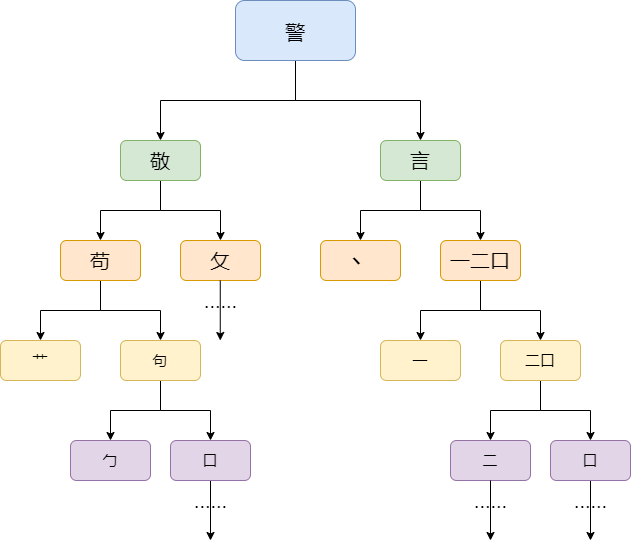
\includegraphics{C:/Users/abget/Study/黑盒攻击/代码部分/汉字拆分结构.png}

\hypertarget{ux6c49ux5b57ux62c6ux5206}{%
\paragraph{汉字拆分}\label{ux6c49ux5b57ux62c6ux5206}}

\hypertarget{ux57faux4e8eux6c49ux5b57ux7ed3ux6784ux4e8cux53c9ux6811ux8fdbux884cux62c6ux5206ux53eaux9009ux53d6ux5de6ux53f3ux90e8ux5206ux8fdbux884cux62c6ux5206}{%
\subparagraph{基于汉字结构二叉树进行拆分,只选取左右部分进行拆分}\label{ux57faux4e8eux6c49ux5b57ux7ed3ux6784ux4e8cux53c9ux6811ux8fdbux884cux62c6ux5206ux53eaux9009ux53d6ux5de6ux53f3ux90e8ux5206ux8fdbux884cux62c6ux5206}}

考虑到汉字中绝大多数是左右结构,比如说"的"是由"白","勺"组成.将其进行横向拆解,人脑能够自动将其进行组合,对文本阅读的影响程度较小.

对于要攻击的汉字,广度优先遍历其结构二叉树.将结构为左右或者左中右等横向可拆分的节点作为遍历节点,将其余的节点作为叶子节点,这样出队序列就是汉字的拆分序列.考虑到组合结构的复杂性,为了简便起见在遇到组合节点的时候认为汉字不可横向拆分,停止遍历.

\begin{verbatim}
String Proceure char_flatten(Hanzi c)

	ret <- ""

	char_queue <- InitQueue(c)

	while not Empty(char_queue):

		char <- Dequeue(char_queue)

		switch char.struct:

			case HanziStructure.左右 or HanziStructure.左中右:

				Enqueue(char_queue,c.sub)

			case HanziStructure.组合:

				ret <- c.c #Stop Flatten Char

				break

			case default:

				ret <- ret + c.c

	return ret
\end{verbatim}

\hypertarget{ux52a8ux6001ux641cux7d22ux5f02ux4f53ux5b57}{%
\paragraph{动态搜索异体字}\label{ux52a8ux6001ux641cux7d22ux5f02ux4f53ux5b57}}

\hypertarget{ux57faux4e8eux6c49ux5b57ux9012ux5f52ux7ed3ux6784ux641cux7d22ux4f18ux5148ux4f7fux7528ux589eux52a0ux504fux65c1ux7684ux6c49ux5b57ux5176ux6b21ux4f7fux7528ux6c49ux5b57ux7684ux90e8ux5206ux7ec4ux4ef6}{%
\subparagraph{基于汉字递归结构搜索.优先使用增加偏旁的汉字,其次使用汉字的部分组件.}\label{ux57faux4e8eux6c49ux5b57ux9012ux5f52ux7ed3ux6784ux641cux7d22ux4f18ux5148ux4f7fux7528ux589eux52a0ux504fux65c1ux7684ux6c49ux5b57ux5176ux6b21ux4f7fux7528ux6c49ux5b57ux7684ux90e8ux5206ux7ec4ux4ef6}}

基于汉字读半边的常见现象,将汉字加上一些偏旁对整体的影响不是很大.如"知"加上"木"形成的"椥"字.因此,基于部首构建了能够根据偏旁查询其更高一级组成的汉字的反向字典.在生成对应异体字的时候,将原汉字作为偏旁在反向字典中进行搜索,得到相应的汉字.若原汉字不作为部件组成汉字,则尝试去掉其偏旁.如"询"去掉"⻈"变成的"旬"依然在一定程度上能够保持其原来的含义.搜索完毕后之后根据笔画近似算法对结果进行排序.

为了让搜索到的异体字更加的接近原来的字体,需要让其余的部分尽可能的简单,占比尽可能的小.因此,首先计算剩余部分在整体字中的占比.对于增加偏旁的异体字来说,由于汉字的部件增加了,笔画数也随之增加.因此其得分为正.对于减少偏旁的异体字来说,相应的,其得分为负.

\[score(C_{mars},C_{origin})=\frac{Count(C_{mars})-Count(C_{origin})}{Count(C_{Origin})}\]

为了让增加或者减少的部分不至于影响到汉字的主体部分,需要对其进行限制.这里选择的过滤条件是增加或者减少的部分不得超过50\%.

\[Filter(C,score)\to \begin{cases}

  True& \text{ if } score<0\ and\ score>-0.5 \\

  True& \text{ if } score>0\ and\ score<1 \\

  False&\ Other\ case

\end{cases}\]

之后对过滤后的汉字得分取绝对值,取得分最小的汉字即为最接近的异体字.

\[C_{target}=Sort(Filter(C,score))\]

\hypertarget{ux52a8ux6001ux751fux6210ux5f62ux8fd1ux5b57}{%
\paragraph{动态生成形近字}\label{ux52a8ux6001ux751fux6210ux5f62ux8fd1ux5b57}}

\hypertarget{ux4ee5ux540cux504fux65c1ux6c49ux5b57ux4e3aux5207ux5165ux53e3ux901aux8fc7ux9012ux5f52ux65b9ux6cd5ux8ba1ux7b97ux6c49ux5b57ux7684ux7ed3ux6784ux52a0ux6743ux76f8ux4f3cux5ea6ux5229ux7528ux52a8ux6001ux89c4ux5212ux7684ux601dux60f3ux52a0ux901fux6c49ux5b57ux76f8ux4f3cux5ea6ux6bd4ux5bf9}{%
\subparagraph{以同偏旁汉字为切入口,通过递归方法计算汉字的结构加权相似度.利用动态规划的思想加速汉字相似度比对}\label{ux4ee5ux540cux504fux65c1ux6c49ux5b57ux4e3aux5207ux5165ux53e3ux901aux8fc7ux9012ux5f52ux65b9ux6cd5ux8ba1ux7b97ux6c49ux5b57ux7684ux7ed3ux6784ux52a0ux6743ux76f8ux4f3cux5ea6ux5229ux7528ux52a8ux6001ux89c4ux5212ux7684ux601dux60f3ux52a0ux901fux6c49ux5b57ux76f8ux4f3cux5ea6ux6bd4ux5bf9}}

该算法主要是利用汉字结构二叉树进行了计算.对于要比较相似度的两个汉字,比较他们的结构是否一致.对于不一致的结构,若其中一个是独体字或者组合字则直接认为他们不相似,返回0作为相似度.否则计算结构枚举的差作为结构偏差系数,然后作为结构一致的计算.\\
对于结构一致的情况如果两者都是独体字,就去直接计算他们的相似度并返回上一级.否则,分别递归计算两个子部件的相似度,然后按笔画数占比求和,乘以结构偏差系数得到两个汉字关于该节点的相似度.

计算完成后排序选取相似度最大的.

\[char\_sim(C_{sim},C_{origin})=\begin{cases}

  cal_(C_{sim},C_{origin})& \text{ if } C_1\ or\ C_2\ is\ Indivisible \\

  & \text{ if } score>0\ and\ score<1 

\end{cases}\]

\begin{figure}
\centering
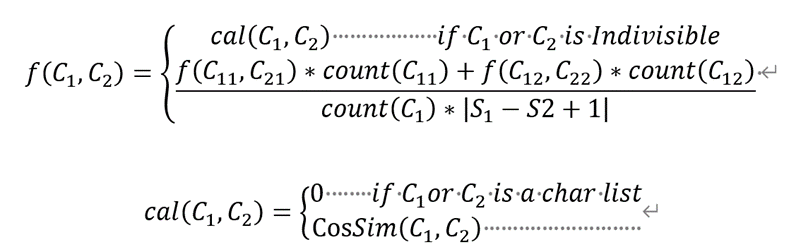
\includegraphics{C:/Users/abget/Study/黑盒攻击/代码部分/other/相似度计算公式.png}
\caption{}
\end{figure}

由于每种中文字体都排除了⼀些字符,仅使用⼀种字体并不能完全解决OOV问题。这样,Text2Img模块除了SimSun之外,会依次使用其他所有兼容的字体,直到可以显示⼀个字符,这样就保证了所有可以显示的字符都被覆盖了。尽管如此,⼀些不可见的字符无法以任何字体显示。这部分是从多个语料库收集的所有字符的⼤约0.02‰,前只使用Macintosh字体库。因此,全黑图像被用来表示这种类型的字符。综上所述,Text2Img模块使模型的输⼊与标消息接收者看到的视觉信息保持⼀致,即该模块确保分类器有机会捕获垃圾邮件发送者想要传播的任何语义。

\#\#\#\#\#

\hypertarget{ux4ee5unicodeux4e3aux6838ux5fc3ux7684ux5f62ux6001ux5b66ux653bux51fb}{%
\subsubsection{以Unicode为核心的形态学攻击}\label{ux4ee5unicodeux4e3aux6838ux5fc3ux7684ux5f62ux6001ux5b66ux653bux51fb}}

现在通行的字符编码是Unicode码,其中主要以UTF-8编码为主.统一码(Unicode).

Unicode是⼀种字符集,旨在标准化文本的电子表示{[}43{]}。截至撰写本文时,它可以表示143,859个字符,涵盖许多不同的语言和符号组。拉丁字母、繁体汉字、数学符号和表情符号等多种多样的字符都可以用Unicode表示。它将每个字符映射到⼀个代码点或数字表示。这些数字代码点,通常用前缀表示U+,可以用多种方式编码,但UTF-8是最常见的。这是⼀种可变长度编码方案,将代码点表示为1-4个字节。字体是描述代码点应如何呈现的字形集合。⼤多数计算机支持持许多不同的字体。不需要字体的每个代码点都有⼀个字形,没有相应字形的代码点通常呈现为``未知''占位符字符。

也叫万国码、单一码,由\href{https://baike.baidu.com/item/统一码联盟/3694574?fromModule=lemma_inlink}{统一码联盟}开发,是\href{https://baike.baidu.com/item/计算机科学领域/12650606?fromModule=lemma_inlink}{计算机科学领域}里的一项业界标准,包括\href{https://baike.baidu.com/item/字符集/946585?fromModule=lemma_inlink}{字符集}、\href{https://baike.baidu.com/item/编码方案/20835369?fromModule=lemma_inlink}{编码方案}等。

统一码是为了解决传统的\href{https://baike.baidu.com/item/字符编码/8446880?fromModule=lemma_inlink}{字符编码}方案的局限而产生的,它为每种\href{https://baike.baidu.com/item/语言/72744?fromModule=lemma_inlink}{语言}中的每个\href{https://baike.baidu.com/item/字符/4768913?fromModule=lemma_inlink}{字符}设定了统一并且唯一的\href{https://baike.baidu.com/item/二进制编码/1758517?fromModule=lemma_inlink}{二进制编码},以满足跨语言、跨平台进行文本转换、处理的要求。

\hypertarget{ux540cux5f62ux5f02ux7801ux5b57}{%
\paragraph{同形异码字}\label{ux540cux5f62ux5f02ux7801ux5b57}}

\hypertarget{ux4f7fux7528unicodeux4e2dux5177ux6709ux7c7bux4f3cux5f62ux6001ux4f46ux662fux7f16ux7801ux4e0dux540cux7684ux6c49ux5b57ux4f5cux4e3aux66ffux6362ux7684ux5bf9ux8c61ux8fdbux884cux653bux51fb}{%
\subparagraph{使用Unicode中具有类似形态但是编码不同的汉字作为替换的对象进行攻击}\label{ux4f7fux7528unicodeux4e2dux5177ux6709ux7c7bux4f3cux5f62ux6001ux4f46ux662fux7f16ux7801ux4e0dux540cux7684ux6c49ux5b57ux4f5cux4e3aux66ffux6362ux7684ux5bf9ux8c61ux8fdbux884cux653bux51fb}}

因为Unicode需要尽可能的收集所有的字符,同时需要兼顾字源分离原则.因此,有大量的同形字符获得了不同的编码.如"用"和"用"两个不同的字符串总是可以由相同的字形序列表示,这些字符串称为\emph{同形异义词}。例如,拉丁语中的``AB''和希腊语中的``AB''是同形异义词。欺骗不仅仅依赖于同形异义词;如果视觉外观在小尺寸或最常见的字体中足够接近,则足以引起问题。有些人广泛使用术语\emph{同形异义词,包括所有视觉上容易混淆的字符串。}

\hypertarget{ux5b57ux7b26ux63d2ux5165ux653bux51fb}{%
\paragraph{字符插入攻击}\label{ux5b57ux7b26ux63d2ux5165ux653bux51fb}}

\hypertarget{ux9009ux62e9ux65e5ux8bedux5e73ux5047ux540dux7247ux5047ux540dux7b49ux5bf9ux6c49ux8bedux8ba4ux8bfbux5f71ux54cdux4e0dux5927ux7684ux5b57ux7b26ux8fdbux884cux63d2ux5165}{%
\subparagraph{选择日语平假名片假名等对汉语认读影响不大的字符进行插入.}\label{ux9009ux62e9ux65e5ux8bedux5e73ux5047ux540dux7247ux5047ux540dux7b49ux5bf9ux6c49ux8bedux8ba4ux8bfbux5f71ux54cdux4e0dux5927ux7684ux5b57ux7b26ux8fdbux884cux63d2ux5165}}

Unicode中存在一些可以附加到其他字符上的字符也就是拼音和音调字符

尽管不可见字符不会生成呈现的字形,但它们仍然代表有效的编码字符。基于文本的NLP模型对编码字节作为输⼊进行操作,因此这些字符将被基于文本的模型``看到'',即使它们没有呈现给⼈类用⼾可感知的任何东西。我们发现这些字节改变了模型输出。当任意注⼊模型的输⼊时,它们通常会降低准确性和运行时间方⾯的性能。当以有针对性的方式注⼊时,它们可用于以所需方式修改输出,并可能连贯地改变许多NLP任务中输出的含义

\hypertarget{unicodeux987aux5e8fux653bux51fb}{%
\paragraph{Unicode顺序攻击}\label{unicodeux987aux5e8fux653bux51fb}}

由于阿拉伯文是从右向左写的,而通行的语言是从左向右书写的.因此Unicode一方面规定了字符的强弱性,另一方面提供了标识字符方向性的字符,同时Unicode也提供了相应的解析算法即Bidi算法.可以反向利用该算法,将一部分汉字的方向进行调换.这样即使文本处理模型滤掉了控制字符,剩下的文本仍然是不可以解读的.

Unicode规范⽀持从左到右和从右到左方向阅读的语⾔中的字符。当混合使用此类脚本时,这将变得⾮常重要。Unicode规范定义了双向(Bidi)算法{[}52{]}以⽀持混合脚本文

图3显示了使用重新排序的攻击示例。在对抗性设置中,Bidi控制字符允许打乱字符的编码顺序⽽不影响字符渲染,从⽽使它们成为⼀种难以察觉的扰动形式

\hypertarget{unicodeemojiux653bux51fb}{%
\paragraph{Unicodeemoji攻击}\label{unicodeemojiux653bux51fb}}

有些emoji可以替换相应的名词,因为现在网络emoji大量流行,可以选取一些形象的emoji对汉字进行替换,例如🀄可以替换中字,🈲替换禁字.

一个合理的选择是直接衡量去除ith字的效果,因为比较去除一个字之前和之后的预测结果可以反映出这个字对分类结果的影响,如图3所示。因此,我们引入了一个评分,确定x中jth词的重要性为。Cwj=Fy(w1,w2,-\/-,wm)-Fy(w1,-\/-,wj-1,wj+1,-\/-,wm)(3)。\\
拟议的评分函数具有以下特性。\\
(1)它能够正确地反映单词对预测的重要性,(2)它在不知道分类模型的参数和结构的情况下计算单词的分数,并且(3)它的计算效率高

\hypertarget{ux5b9eux9a8cux7ed3ux679c}{%
\subsection{实验结果}\label{ux5b9eux9a8cux7ed3ux679c}}

我们使用四个指标,即编辑距离、雅卡德相似系数、欧氏距离和语义相似度,来评估生成的对抗性文本的效用。具体来说,编辑距离和Jaccard相似系数是在原始文本上计算的,而欧氏距离和语义相似度是在单词向量上计算的。\\
编辑距离。编辑距离是通过计算将一个字符串转换为另一个字符串所需的最小操作数来量化两个字符串(例如,句子)的不同程度的方法。具体来说,编辑距离的不同定义使用不同的字符串操作集。在我们的实验中,我们使用最常见的度量,即列文斯坦距离,其操作包括删除、插入和替换字符串中的字符。\\
雅卡德相似性系数。雅卡德相似系数是一个用于测量有限样本集的相似性和多样性的统计数字。它被定义为交集的大小除以样本集的联合体的大小。

们用词的移动距离WMD来衡量对抗性例子的质量。WMD表示从句子向量p中的词pi到句子向量q中的词qj的整体移动距离,其中Ti,j是移动距离的权重,d是向量之间的欧氏距离,因此WMD可以表述为:。

\hypertarget{ux591aux6a21ux578bux8fd0ux884cux7ed3ux679c}{%
\subsubsection{多模型运行结果}\label{ux591aux6a21ux578bux8fd0ux884cux7ed3ux679c}}

验证结果依次为\\
2000个的准确度下降程度运行时间比较\\
bert.zh\textasciitilde 亚马逊\\
Structbert-tiny\textasciitilde 豆瓣轮胎\\
Paddle-nano\textasciitilde paddle

拆分攻击方式再来一遍,在亚马逊数据集上做测试.

零影响替换\textasciitilde bidi算法攻击,Unicode同形码攻击和空白插入攻击,emoji替换\\
低影响替换\textasciitilde 汉字拆解攻击和汉字增减攻击\\
高影响替换\textasciitilde 形近字替换攻击

判断指标,对于零影响的不做判断,对于低和高影响的用问卷判断,找10个人.

用贝叶斯模型和不用贝叶斯模型进行判断

随机和词重要性比较

和PWW模型做为基线模型进行比较?

\begin{figure}
\centering
\includegraphics{https://pic3.zhimg.com/v2-2891cdff9038c659d54c84aee6eba6ca_r.jpg}
\caption{}
\end{figure}

表二总结了IMDB和MR数据集上白盒攻\\
击的主要结果和基线方法的性能比较,其中表二的第三列显示了非对抗性设置下的原始模型准确性。我们没有给出在白盒设置下生成一个对抗性例子的平均时间,因为模型是离线的,而且攻击的效率很高(例如,在一秒钟内生成数百个对抗性文本)。从表二中,我们可以看到,随机选择要改变的词(即表二中的随机)对最终结果几乎没有任何影响。这意味着随机改变单词不会欺骗分类器,选择重要的单词进行修改是成功攻击的必要条件。从表二中,我们还可以看到,标模型在非对抗性设置中都表现得相当好。然而,由TEXTBUGGER生成的对抗性文本对这些模型的攻击成功率仍然很高。此外,线性模型比深度学习模型更容易受到对抗性文本的影响。具体来说,TEXTBUGGER只扰动了几个词就达到了很高的攻击成功率,并且对所有\\
模型的表现都比基线算法好很多,如表二所示。例如,在IMDB数据集上针对LR模型实现95.2\%的成功率时,它只扰乱了一个样本的4.9\%的单词,而所有基线在这种情况下实现的成功率不超过42\%。由于IMDB数据集的平均长度为215.63个单词,TEXTBUGGER只对一个样本进行了约10个单词的扰动,就能进行成功的攻击

\hypertarget{ux603bux7ed3ux548cux5c55ux671b}{%
\subsection{总结和展望}\label{ux603bux7ed3ux548cux5c55ux671b}}

\hypertarget{ux4f18ux52bf}{%
\subsubsection{优势}\label{ux4f18ux52bf}}

\hypertarget{ux4e0dux8db3}{%
\subsubsection{不足}\label{ux4e0dux8db3}}

\hypertarget{ux7ee7ux7eedux52aaux529bux7684ux65b9ux5411}{%
\subsubsection{继续努力的方向}\label{ux7ee7ux7eedux52aaux529bux7684ux65b9ux5411}}

{[}\href{https://www-unicode-org.translate.goog/reports/tr39/tr39-22.html?_x_tr_sl=auto\&_x_tr_tl=zh-CN\&_x_tr_hl=zh-CN\#confusables}{confusables}{]}中的数据提供了一种机制,用于确定两个字符串何时在视觉上容易混淆。随着时间的推移,这些文件中的数据可能会得到完善和扩展。有关随时间推移处理修改的信息,请参阅Unicode技术报告\#36``Unicode安全注意事项''{[}\href{https://www-unicode-org.translate.goog/reports/tr39/tr39-22.html?_x_tr_sl=auto\&_x_tr_tl=zh-CN\&_x_tr_hl=zh-CN\#UTR36}{UTR36{]}中的}\emph{第2.9.1节``向后兼容性}''和本文档的\href{https://www-unicode-org.translate.goog/reports/tr39/tr39-22.html?_x_tr_sl=auto\&_x_tr_tl=zh-CN\&_x_tr_hl=zh-CN\#Migration}{``迁移''部分。}

收集用于检测网守易混淆字符串的数据前不是本文档中易混淆检测机制的标。有关详细信息,请参阅第2节,{[}\href{https://www-unicode-org.translate.goog/reports/tr39/tr39-22.html?_x_tr_sl=auto\&_x_tr_tl=zh-CN\&_x_tr_hl=zh-CN\#UTR36}{UTR36{]}中的}\emph{视觉安全问题}。

数据提供了从源字符到原型的映射。原型应该被认为是一个或多个符号类别的序列,其中每个类别都有一个示例字符。例如,字符U+0153(œ),拉丁小写连字OE,其原型由两个符号类组成:一个是示例字符U+006F(o),另一个是示例字符U+0065(e).如果输入字符没有在数据文件中明确定义的原型,则假定原型由以输入字符作为示例字符的符号类组成。

对于输入字符串X,将\href{https://www-unicode-org.translate.goog/reports/tr39/tr39-22.html?_x_tr_sl=auto\&_x_tr_tl=zh-CN\&_x_tr_hl=zh-CN\#def-skeleton}{骨架}(X)定义为字符串的以下转换:

\begin{enumerate}
\def\labelenumi{\arabic{enumi}.}
\item
  {[}将X转换为NFD格式,如\href{https://www-unicode-org.translate.goog/reports/tr39/tr39-22.html?_x_tr_sl=auto\&_x_tr_tl=zh-CN\&_x_tr_hl=zh-CN\#UAX15}{UAX15}{]}中所述。
\item
  根据指定数据连接X中每个字符的原型,生成一串示例字符。
\item
  重新申请NFD。
\end{enumerate}

当且仅当skeleton(X)=skeleton(Y)时,字符串X和Y被定义为可\href{https://www-unicode-org.translate.goog/reports/tr39/tr39-22.html?_x_tr_sl=auto\&_x_tr_tl=zh-CN\&_x_tr_hl=zh-CN\#def-confusable}{混淆。}这缩写为X≅Y。

这种机制对数据施加了传递性,因此如果X≅Y和Y≅Z,则X≅Z。可以通过提供给定字符之间的度量来提供更复杂的混淆检测,指示它们的``接近度''。然而,这在计算上要昂贵得多,并且需要更复杂的数据,因此此时选择了更简单的机制。这意味着在某些情况下,测试可能过于包容。

Unicode标准提供可用于确定字符脚本和检测混合脚本文本的信息。脚本的确定是根据\emph{UAX\#24,Unicode脚本属性}{[}\href{https://www-unicode-org.translate.goog/reports/tr39/tr39-22.html?_x_tr_sl=auto\&_x_tr_tl=zh-CN\&_x_tr_hl=zh-CN\#UAX24}{UAX24}{]},使用来自Unicode字符数据库{[}\href{https://www-unicode-org.translate.goog/reports/tr39/tr39-22.html?_x_tr_sl=auto\&_x_tr_tl=zh-CN\&_x_tr_hl=zh-CN\#UCD}{UCD}{]}的数据。

通过以下两个修改将角色的\href{https://www-unicode-org.translate.goog/reports/tr39/tr39-22.html?_x_tr_sl=auto\&_x_tr_tl=zh-CN\&_x_tr_hl=zh-CN\#def-augmented-script-set}{扩充脚本集定义为角色的Script\_Extensions。}

\begin{enumerate}
\def\labelenumi{\arabic{enumi}.}
\item
  包含多个脚本的书写系统的条------Hanb(带有Bopomofo的汉字)、Jpan(日语)和Kore(韩语)------是根据以下规则添加的。

  \begin{enumerate}
  \def\labelenumii{\arabic{enumii}.}
  \item
    如果Script\_Extensions包含Hani(Han),请添加Hanb、Jpan和Kore。
  \item
    如果Script\_Extensions包含Hira(平假名),请添加Jpan。
  \item
    如果Script\_Extensions包含假名(片假名),请添加Jpan。
  \item
    如果Script\_Extensions包含Hang(Hangul),请添加Kore。
  \item
    如果Script\_Extensions包含Bopo(Bopomofo),则添加Hanb。
  \end{enumerate}
\item
  包含Zyyy(通用)或Zinh(继承)的集合被视为\textbf{ALL},即所有脚本值的集合。
\end{enumerate}

Script\_Extensions数据来自Unicode字符数据库{[}\href{https://www-unicode-org.translate.goog/reports/tr39/tr39-22.html?_x_tr_sl=auto\&_x_tr_tl=zh-CN\&_x_tr_hl=zh-CN\#UCD}{UCD}{]}。有关Script\_Extensions属性和Jpan、Kore和Hanb的更多信息,请参阅\emph{UAX\#24,Unicode脚本属性}{[}\href{https://www-unicode-org.translate.goog/reports/tr39/tr39-22.html?_x_tr_sl=auto\&_x_tr_tl=zh-CN\&_x_tr_hl=zh-CN\#UAX24}{UAX24}{]}。

将字符串\href{https://www-unicode-org.translate.goog/reports/tr39/tr39-22.html?_x_tr_sl=auto\&_x_tr_tl=zh-CN\&_x_tr_hl=zh-CN\#def-resolved-script-set}{的解析脚本集}定义为字符串中所有字符的扩充脚本集的交集。

如果解析的脚本集为空,则字符串定义为\href{https://www-unicode-org.translate.goog/reports/tr39/tr39-22.html?_x_tr_sl=auto\&_x_tr_tl=zh-CN\&_x_tr_hl=zh-CN\#def-mixed-script}{混合脚本;}如果解析的脚本集为非空,则字符串定义为\href{https://www-unicode-org.translate.goog/reports/tr39/tr39-22.html?_x_tr_sl=auto\&_x_tr_tl=zh-CN\&_x_tr_hl=zh-CN\#def-single-script}{单脚本。}

请注意,术语``\emph{单}脚本字符串''可能会造成混淆。\emph{这意味着解析的脚本集中至少}有一个脚本,而不是只有\emph{一个}.例如,字符串``〆切''是单文字,因为它在解析的文字集中有\emph{四个}文字\{Hani,Hanb,Jpan,Kore\}。

参考文献区

\url{https://www.unicode.org/reports/tr39/tr39-22.html}

\url{https://www.unicode.org/reports/tr36/tr36-15.html}

\end{document}
